% Auto-generated by code/s9c_latex_includes.py (experiment-bridge).
% The MVA template loads no float package, so all floats use [!htbp].

\begin{figure}[!htbp]
    \centering
    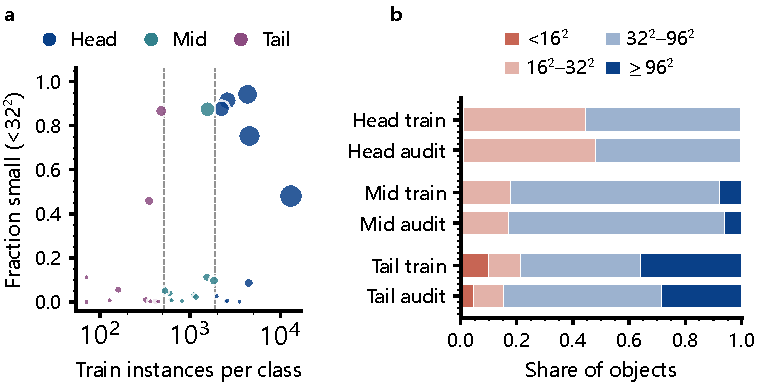
\includegraphics[width=0.98\textwidth,height=0.8\textheight,keepaspectratio]{figures/fig_size_frequency.pdf}
    \caption{Size is a class property, not a frequency property (RicePest-30, 640-long-edge frame). Left: one point per class, train instances versus the fraction of its objects smaller than $32^2$; point area grows with the number of small objects of that class in the audit set; dashed lines separate the head, mid and tail tertiles. The large tail point is \textit{Jacobiasca formosana}. Right: size composition of each stratum in train and in the audit set.}
    \label{fig:size-frequency}
\end{figure}

\begin{figure}[!htbp]
    \centering
    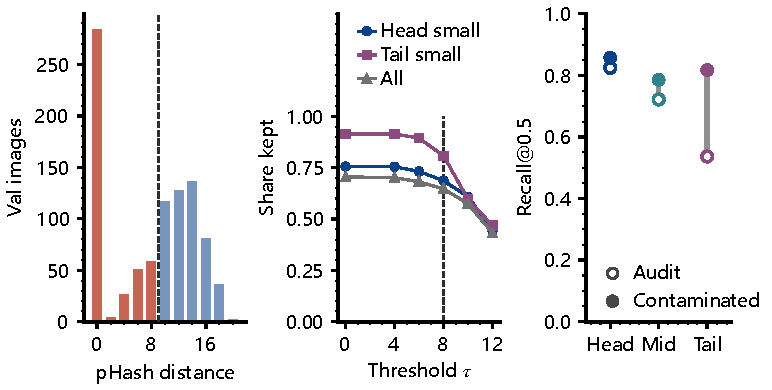
\includegraphics[width=0.98\textwidth,height=0.8\textheight,keepaspectratio]{figures/fig_leakage.pdf}
    \caption{Leakage in the published split. Left: pHash distance from each validation image to its nearest training image (red: at or below the frozen threshold $\tau=8$). Middle: share of validation objects kept in the group-disjoint audit set as $\tau$ varies. Right: recall@0.5 of the frozen pipeline on audit images (hollow) and on contaminated validation images (filled), per stratum.}
    \label{fig:leakage}
\end{figure}

\begin{figure}[!htbp]
    \centering
    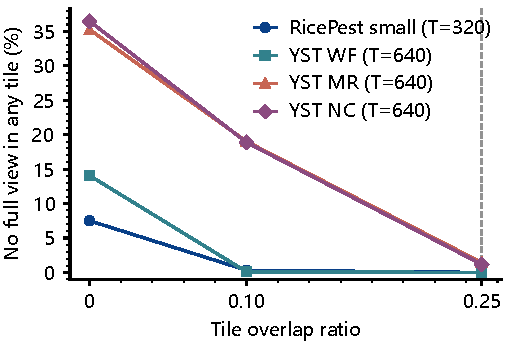
\includegraphics[width=0.65\textwidth,height=0.8\textheight,keepaspectratio]{figures/fig_truncation_control.pdf}
    \caption{Literal truncation (no full view in any tile) against tile overlap: negative control at the frozen overlap 0.25 (dashed) and positive control at overlap 0. RicePest-30 small objects of the audit set ($T$=320 in the 640 frame) and YST objects per class (native $T$=640).}
    \label{fig:truncation}
\end{figure}

\begin{figure}[!htbp]
    \centering
    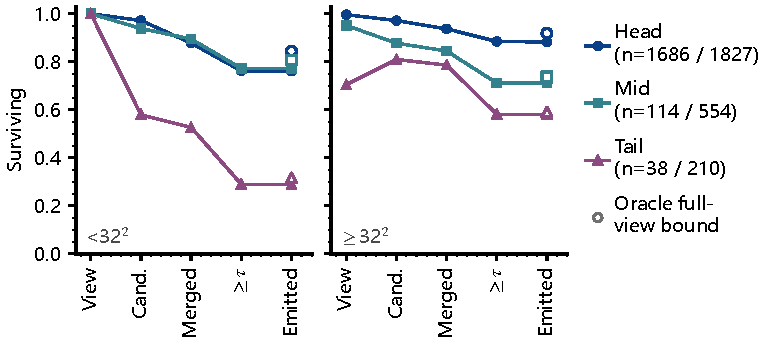
\includegraphics[width=0.98\textwidth,height=0.8\textheight,keepaspectratio]{figures/fig_stage_survival.pdf}
    \caption{Stage-survival profile of the per-object ledger on the audit set (YOLO11n). Left: objects smaller than $32^2$; right: larger objects. Hollow markers: oracle full-view read-out (baseline detections plus every same-class candidate scoring at least 0.25 in a view that holds the whole object).}
    \label{fig:stage-survival}
\end{figure}

\begin{figure}[!htbp]
    \centering
    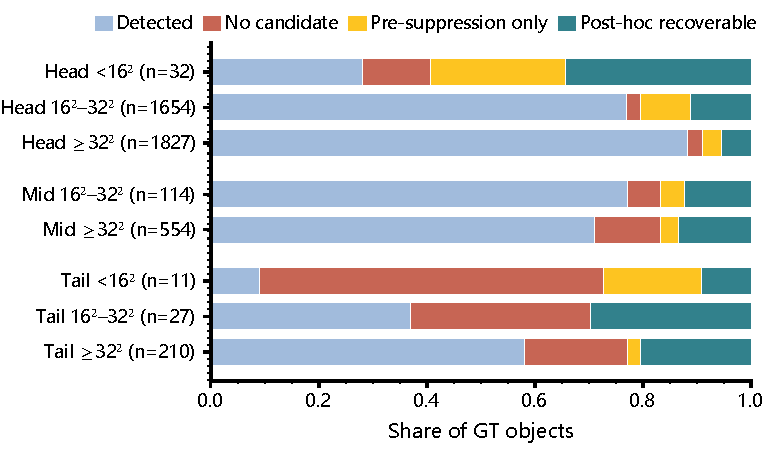
\includegraphics[width=0.98\textwidth,height=0.8\textheight,keepaspectratio]{figures/fig_partition.pdf}
    \caption{Recovery-ceiling partition of every audit object (YOLO11n, SAHI $T$=320, overlap 0.25). Each bar splits the objects of one stratum and size bin into detected, no candidate, pre-suppression only and post-hoc recoverable.}
    \label{fig:partition}
\end{figure}

\begin{figure}[!htbp]
    \centering
    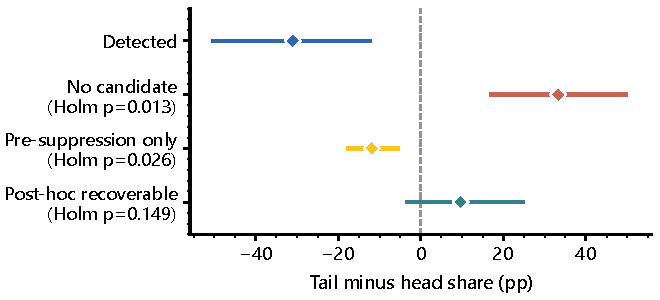
\includegraphics[width=0.85\textwidth,height=0.8\textheight,keepaspectratio]{figures/fig_contrast.pdf}
    \caption{Size-matched frequency contrast: share of each outcome among tail-small objects minus the share among head-small objects re-weighted to the tail size mix (percentage points; bars: 95\% cluster-bootstrap CI over audit groups; Holm-adjusted $p$ from exact class-label permutation).}
    \label{fig:contrast}
\end{figure}

\begin{figure}[!htbp]
    \centering
    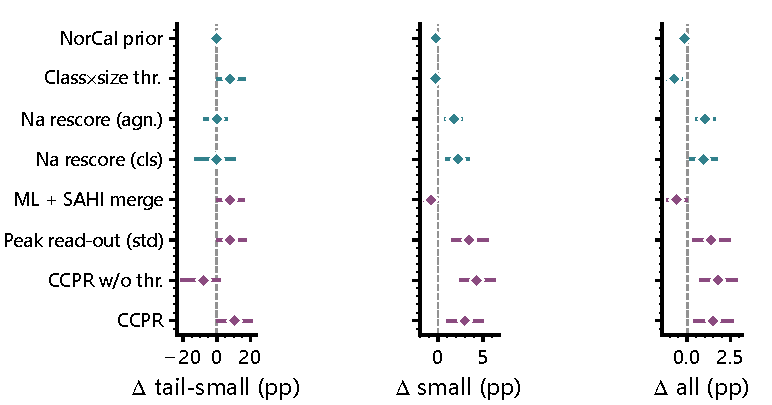
\includegraphics[width=0.98\textwidth,height=0.8\textheight,keepaspectratio]{figures/fig_methods.pdf}
    \caption{Same-dump post-processing against the frozen SAHI baseline at matched false positives: paired difference in recall@0.5 (percentage points, 95\% cluster-bootstrap CI). Left to right: tail-small (38 objects), small (1838) and all (4429) audit objects. Teal: post-hoc rescoring/calibration; violet: read-out changes.}
    \label{fig:methods}
\end{figure}

\begin{figure}[!htbp]
    \centering
    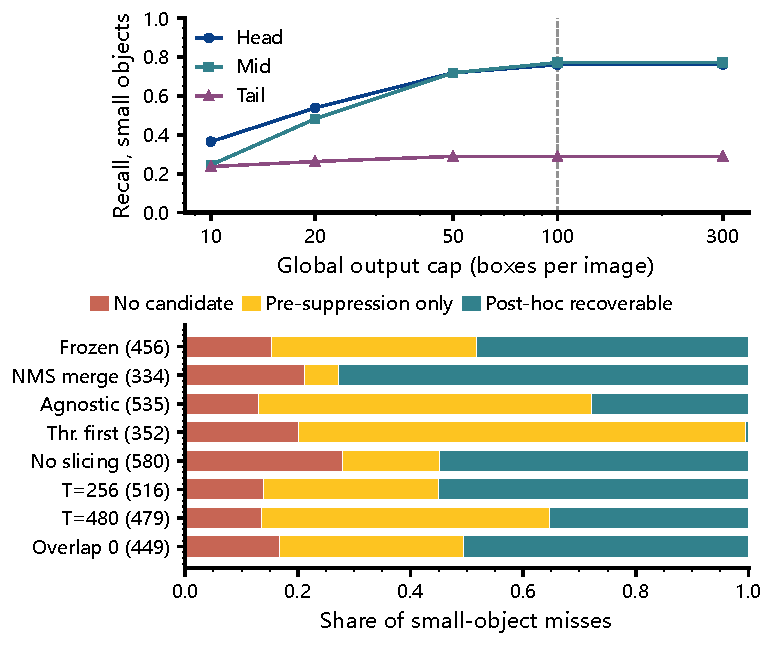
\includegraphics[width=0.98\textwidth,height=0.8\textheight,keepaspectratio]{figures/fig_sensitivity.pdf}
    \caption{Sensitivity of the ledger. Top: recall of small objects per stratum against the global output cap (frozen cap 100 dashed). Bottom: composition of small-object misses under the frozen pipeline and alternative read-outs and tilings (number of misses in brackets).}
    \label{fig:sensitivity}
\end{figure}

\begin{figure}[!htbp]
    \centering
    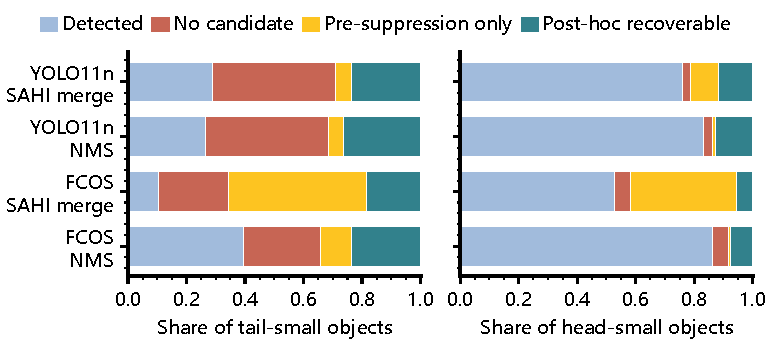
\includegraphics[width=0.98\textwidth,height=0.8\textheight,keepaspectratio]{figures/fig_detectors.pdf}
    \caption{Cross-detector check: outcome shares of tail-small (left, 38 objects) and head-small (right, 1686 objects) audit objects for YOLO11n and FCOS-ResNet50-FPN under the frozen SAHI merge (GREEDYNMM-IOS at the 0.01 floor) and under an NMS-IoU 0.5 merge.}
    \label{fig:detectors}
\end{figure}

\begin{figure}[!htbp]
    \centering
    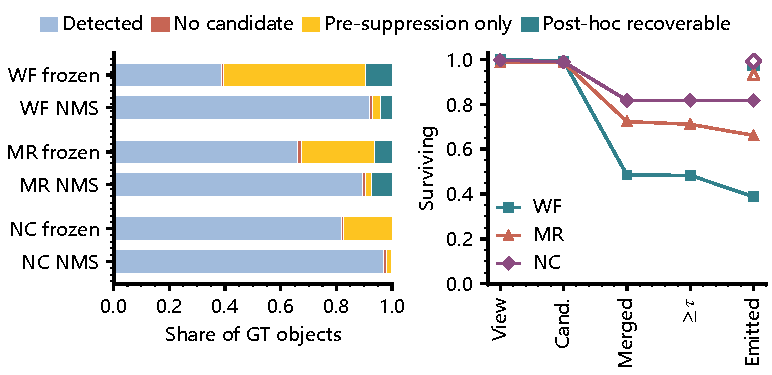
\includegraphics[width=0.98\textwidth,height=0.8\textheight,keepaspectratio]{figures/fig_yst.pdf}
    \caption{Native-resolution source re-check on Yellow Sticky Traps (85 held-out test images; WF 1882, MR 584, NC 257 objects). Left: outcome partition per class under the frozen pipeline and under an NMS read-out with a 300-box cap. Right: stage survival per class under the frozen pipeline; hollow markers: oracle full-view read-out.}
    \label{fig:yst}
\end{figure}

\begin{figure}[!htbp]
    \centering
    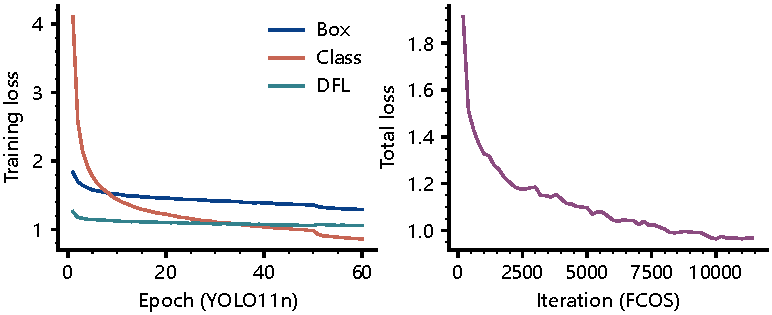
\includegraphics[width=0.98\textwidth,height=0.8\textheight,keepaspectratio]{figures/fig_training.pdf}
    \caption{Training losses of the two frozen RicePest-30 detectors (no validation data were used for checkpoint selection).}
    \label{fig:training}
\end{figure}

% ---- fig_arch (HTML schematic; the per-object stage ledger instrument, paper-figure-html) ----
\begin{figure}[!htbp]
    \centering
    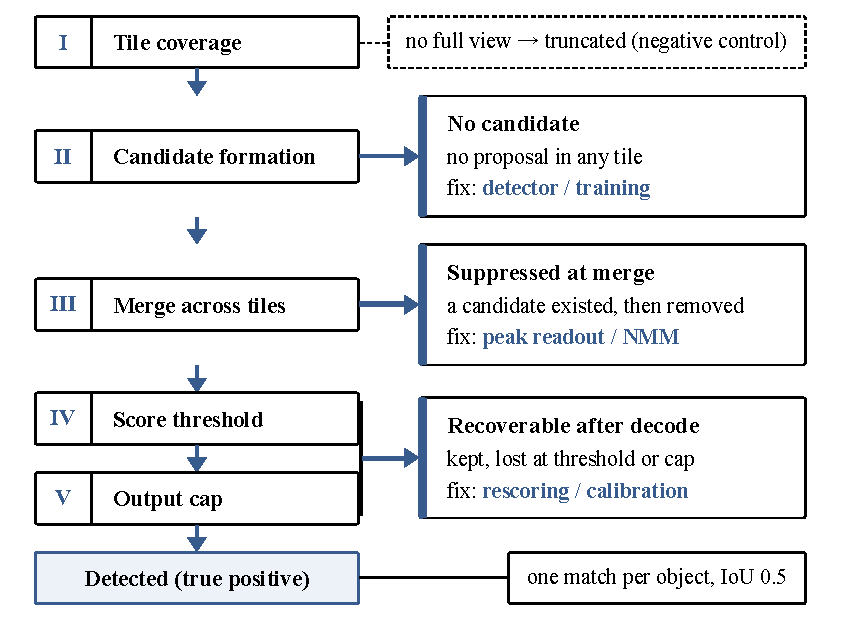
\includegraphics[width=0.92\textwidth,height=0.8\textheight,keepaspectratio]{figures/fig_arch.pdf}
    \caption{The per-object stage ledger: an object traverses tile coverage, candidate formation, cross-tile merge, score threshold and output cap, and a miss is assigned to the stage that first removes it. The three recovery-ceiling categories (no candidate, suppressed at merge, recoverable after decode) name the class of fix each miss admits; failing coverage is literal truncation, the negative control.}
    \label{fig:arch}
\end{figure}

% ---- tables (booktabs; generated by code/s9_tables.py)
\begin{table}[!htbp]
\centering
\scriptsize
\caption{Frozen configuration (written to \texttt{configs/prereg\_frozen.json} before any detector output existed).}
\label{tab:config}
\begin{tabular}{lp{0.72\linewidth}}
\toprule
Component & Setting \\
\midrule
Detector A & YOLO11n, COCO init, 640 input, 60 epochs, batch 16, seed 0, last checkpoint (no selection on validation) \\
Detector B & FCOS-ResNet50-FPN (torchvision), COCO init, 640, 6 epochs, batch 4, last checkpoint \\
Reference frame & image resized to 640-pixel long edge; size bins on box area in this frame \\
Views & full image + SAHI tiles $T$=320, overlap 0.25 (stride 240); every view letterboxed to 640 \\
Candidate dump & per-view score floor 0.01, per-view NMS IoU 0.7, max 300 boxes; single label per anchor \\
Read-out (merge) & SAHI GREEDYNMM, IOS 0.5, class-aware, on the floor-level dump \\
Operating point & score $\geq$0.25, at most 100 boxes per image; matching IoU $\geq$0.5, one-to-one \\
Grouping & 64-bit pHash, Hamming $\leq$8 with a shared class, or identical MD5; connected components \\
Audit set & validation images whose component holds no training image \\
Statistics & cluster percentile bootstrap over audit groups (2,000), Holm over 3 categories, class-label permutation (10,000) \\
Weights hash & YOLO11n bcde46c946b0; FCOS f41271c04f8e \\
\bottomrule
\end{tabular}
\end{table}

\begin{table}[!htbp]
\centering
\small
\caption{Train/validation near-duplicate grouping and the resulting group-disjoint audit set (RicePest-30, 890 frame-consistent validation images).}
\label{tab:leakage}
\resizebox{\linewidth}{!}{%
\begin{tabular}{rrrrrrr}
\toprule
$\tau$ & Contaminated val & Audit images & Audit groups & Head-small & Mid-small & Tail-small (groups) \\
\midrule
0 & 249 & 641 & 626 & 1856 & 146 & 43 (30) \\
4 & 274 & 616 & 601 & 1854 & 146 & 43 (30) \\
6 & 315 & 575 & 559 & 1797 & 136 & 42 (29) \\
8$^{\ast}$ & 367 & 523 & 508 & 1686 & 114 & 38 (27) \\
10 & 444 & 446 & 431 & 1494 & 81 & 28 (21) \\
12 & 555 & 335 & 325 & 1097 & 49 & 22 (17) \\
\bottomrule
\end{tabular}}
\par\smallskip\parbox{0.95\linewidth}{\footnotesize $\tau$: 64-bit pHash Hamming threshold for a near-duplicate link (links also require a shared class; byte-identical files are always linked). $^{\ast}$Frozen setting. 285 of 933 validation images have a training image at pHash distance 0; 279 byte-identical (MD5) groups span both splits.}
\end{table}

\begin{table}[!htbp]
\centering
\small
\caption{Literal truncation: objects with no full view in any SAHI tile (counts truncated/total). RicePest-30 rows count small objects ($<32^2$ in the 640-long-edge frame).}
\label{tab:truncation}
\resizebox{\linewidth}{!}{%
\begin{tabular}{llrrrrr}
\toprule
Data & $T$/stride & Train small & Val small & Audit small & Audit tail-small & Seam-cut (\%) \\
\midrule
RicePest-30 & 320/240$^{\ast}$ & 0/21048 & 0/2680 & 0/1838 & 0/38 & 26.3 \\
RicePest-30 & 320/288 & 67/21048 & 10/2680 & 6/1838 & 0/38 & 26.2 \\
RicePest-30 & 320/320 & 1614/21048 & 214/2680 & 138/1838 & 3/38 & 19.3 \\
RicePest-30 & 256/192 & 0/21048 & 0/2680 & 0/1838 & 0/38 & 41.0 \\
RicePest-30 & 480/360 & 0/21048 & 0/2680 & 0/1838 & 0/38 & 12.5 \\
YST (native) & 640/480$^{\ast}$ & \multicolumn{4}{c}{31/8114 all objects (WF 0, MR 23, NC 8)} & 45.9 \\
YST (native) & 640/576 & \multicolumn{4}{c}{444/8114 all objects (WF 6, MR 308, NC 130)} & 38.6 \\
YST (native) & 640/640 & \multicolumn{4}{c}{1639/8114 all objects (WF 817, MR 571, NC 251)} & 25.4 \\
YST (native) & 512/384 & \multicolumn{4}{c}{147/8114 all objects (WF 0, MR 102, NC 45)} & 55.9 \\
\bottomrule
\end{tabular}}
\par\smallskip\parbox{0.95\linewidth}{\footnotesize Seam-cut: share of objects crossed by at least one tile border (they still have a full view in a neighbouring tile). $^{\ast}$Frozen configuration. Overlap 0 is a positive control: it removes the redundancy that guarantees a full view.}
\end{table}

\begin{table}[!htbp]
\centering
\footnotesize
\caption{Recovery-ceiling partition of missed objects (YOLO11n).}
\label{tab:partition}
\begin{tabular}{lrrrrrr}
\toprule
Stratum, size & $N$ (groups) & Recall (\%) & Misses & No cand. & Pre-supp. & Post-hoc \\
\midrule
Tail $<32^2$ (primary) & 38 (27) & 28.9 & 27 & 16 (59) & 2 (7) & 9 (33) \\
\quad 95\% CI & & [12, 49] & & [41, 78] & [0, 18] & [17, 55] \\
\quad Tail $<16^2$ & 11 (5) & 9.1 & 10 & 7 & 2 & 1 \\
\quad Tail $16^2$--$32^2$ & 27 (24) & 37.0 & 17 & 9 (53) & 0 (0) & 8 (47) \\
Mid $<32^2$ & 114 (29) & 77.2 & 26 & 7 (27) & 5 (19) & 14 (54) \\
Head $<32^2$ & 1686 (257) & 76.1 & 403 & 47 (12) & 159 (39) & 197 (49) \\
\quad 95\% CI & & [74, 79] & & [8, 16] & [32, 46] & [42, 56] \\
Tail $\geq 32^2$ & 210 (156) & 58.1 & 88 & 40 (45) & 5 (6) & 43 (49) \\
Mid $\geq 32^2$ & 554 (251) & 71.1 & 160 & 67 (42) & 19 (12) & 74 (46) \\
Head $\geq 32^2$ & 1827 (332) & 88.2 & 215 & 50 (23) & 65 (30) & 100 (47) \\
All objects & 4429 (508) & 79.3 & 919 & 227 (25) & 255 (28) & 437 (48) \\
\bottomrule
\end{tabular}
\par\smallskip\parbox{0.95\linewidth}{\footnotesize Group-disjoint audit set, frozen YOLO11n + SAHI ($T$=320, overlap 0.25, GREEDYNMM/IOS 0.5 at the 0.01 floor), operating point score $\geq$0.25 and 100 boxes per image. Miss columns: count (\% of misses); CI rows: 95\% cluster-bootstrap CI over audit groups; rates and CIs are omitted when a cell has $<$10 events or $<$5 groups. Size-matched contrast (tail-small vs head-small standardized to the tail size mix): no-candidate share difference 33.3 pp [16.7, 50.0], Holm $p$=0.013; pre-suppression-only -11.9 pp [-18.0, -5.2], Holm $p$=0.026; post-hoc-recoverable 9.6 pp [-3.7, 25.1], Holm $p$=0.149.}
\end{table}

\begin{table}[!htbp]
\centering
\footnotesize
\caption{Recovery-ceiling partition of missed objects (FCOS).}
\label{tab:partition-fcos}
\begin{tabular}{lrrrrrr}
\toprule
Stratum, size & $N$ (groups) & Recall (\%) & Misses & No cand. & Pre-supp. & Post-hoc \\
\midrule
Tail $<32^2$ (primary) & 38 (27) & 10.5 & 34 & 9 (26) & 18 (53) & 7 (21) \\
\quad 95\% CI & & [2, 21] & & [7, 47] & [32, 76] & [10, 34] \\
\quad Tail $<16^2$ & 11 (5) & 18.2 & 9 & 6 & 3 & 0 \\
\quad Tail $16^2$--$32^2$ & 27 (24) & 7.4 & 25 & 3 (12) & 15 (60) & 7 (28) \\
Mid $<32^2$ & 114 (29) & 45.6 & 62 & 5 (8) & 51 (82) & 6 (10) \\
Head $<32^2$ & 1686 (257) & 52.7 & 797 & 92 (12) & 610 (77) & 95 (12) \\
\quad 95\% CI & & [48, 57] & & [9, 14] & [71, 82] & [8, 16] \\
Tail $\geq 32^2$ & 210 (156) & 37.1 & 132 & 9 (7) & 112 (85) & 11 (8) \\
Mid $\geq 32^2$ & 554 (251) & 37.5 & 346 & 15 (4) & 302 (87) & 29 (8) \\
Head $\geq 32^2$ & 1827 (332) & 51.2 & 892 & 23 (3) & 842 (94) & 27 (3) \\
All objects & 4429 (508) & 48.9 & 2263 & 153 (7) & 1935 (86) & 175 (8) \\
\bottomrule
\end{tabular}
\par\smallskip\parbox{0.95\linewidth}{\footnotesize Group-disjoint audit set, frozen FCOS + SAHI ($T$=320, overlap 0.25, GREEDYNMM/IOS 0.5 at the 0.01 floor), operating point score $\geq$0.25 and 100 boxes per image. Miss columns: count (\% of misses); CI rows: 95\% cluster-bootstrap CI over audit groups; rates and CIs are omitted when a cell has $<$10 events or $<$5 groups. Size-matched contrast (tail-small vs head-small standardized to the tail size mix): no-candidate share difference 11.1 pp [-3.8, 26.7], Holm $p$=0.006; pre-suppression-only 1.1 pp [-22.3, 24.9], Holm $p$=0.996; post-hoc-recoverable 13.6 pp [1.4, 27.6], Holm $p$=0.013.}
\end{table}

\begin{table}[!htbp]
\centering
\scriptsize
\caption{Same-dump post-processing methods on the audit set (YOLO11n; parameters fit by 5-fold group cross-fitting).}
\label{tab:methods}
\resizebox{\linewidth}{!}{%
\begin{tabular}{lrrrrrrrrr}
\toprule
Method & \multicolumn{4}{c}{Own operating point} & \multicolumn{5}{c}{Matched false positives} \\ \cmidrule(lr){2-5}\cmidrule(lr){6-10} & R all & Tail-small & P head & FP & R all & R head-small & Tail-small & Recovered P/H/N & Lost \\
\midrule
SAHI baseline (frozen) & 79.3 & 11/38 & 54.6 & 3671 & 79.3 & 76.1 & 11/38 & 0/0/0 & 0 \\
NorCal-style prior correction & 79.1 & 11/38 & 55.1 & 3621 & 79.1 & 75.9 & 11/38 & 0/2/0 & 9 \\
Class$\times$size thresholds & 69.1 & 11/38 & 68.9 & 1715 & 78.5 & 75.7 & 14/38 & 0/31/0 & 64 \\
Na-style rescoring, class-agnostic & 77.5 & 10/38 & 61.3 & 2766 & 80.3 & 77.9 & 11/38 & 0/103/0 & 57 \\
Na-style rescoring, per class & 74.9 & 9/38 & 65.2 & 2151 & 80.2 & 78.4 & 11/38 & 0/143/0 & 102 \\
Multi-label evidence + SAHI merge + thr. & 69.2 & 12/38 & 68.9 & 1772 & 78.6 & 75.2 & 14/38 & 2/36/20 & 85 \\
Peak read-out on std evidence + thr. & 72.3 & 10/38 & 67.1 & 2016 & 80.6 & 80.1 & 14/38 & 201/13/0 & 153 \\
CCPR without class$\times$size thr. & 83.4 & 11/38 & 51.4 & 4497 & 81.0 & 81.1 & 8/38 & 207/3/1 & 132 \\
CCPR (multi-label peak read-out + thr.) & 72.6 & 11/38 & 67.1 & 2073 & 80.7 & 79.6 & 15/38 & 200/20/16 & 170 \\
\bottomrule
\end{tabular}}
\par\smallskip\parbox{0.95\linewidth}{\footnotesize R: recall@0.5 (\%); P head: precision of emitted head-class boxes (\%); tail-small: detected/total. Matched FP: one global threshold per method chosen so that its total false positives do not exceed the baseline's. Recovered P/H/N: baseline misses recovered at matched FP, by the baseline's recovery-ceiling category (pre-suppression only / post-hoc recoverable / no candidate); Lost: baseline detections no longer detected.}
\end{table}

\begin{table}[!htbp]
\centering
\scriptsize
\caption{Pre-registered go/no-go test of CCPR against class$\times$size threshold calibration (audit set, YOLO11n).}
\label{tab:ccpr}
\resizebox{\linewidth}{!}{%
\begin{tabular}{lrrrrrr}
\toprule
Comparison & Extra tail-small TP & $\Delta$ tail-small recall, pp [95\% CI] & $\Delta$ head recall, pp (one-sided 95\% LB) & NI margin (pp) & Criteria 1/2/3 & Decision \\
\midrule
Own operating points & +0 & +0.0 [-11.1, 9.1] & +3.7 (+2.7) & 1 & no/yes/no & NO-GO \\
Matched head precision & -1 & -2.6 [-13.8, 4.8] & +0.9 (-0.4) & 1 & no/yes/no & NO-GO \\
Matched false positives & +1 & +2.6 [-6.1, 10.8] & +2.7 (+1.7) & 1 & no/yes/no & NO-GO \\
\bottomrule
\end{tabular}}
\par\smallskip\parbox{0.95\linewidth}{\footnotesize Criteria: (1) at least 5 additional tail-small true positives; (2) head non-inferiority, one-sided paired cluster bootstrap lower bound above $-$margin; (3) 95\% cluster-bootstrap CI of the tail-small recall difference excludes 0. All three must hold for GO.}
\end{table}

\begin{table}[!htbp]
\centering
\scriptsize
\caption{Sensitivity of recall and of the recovery-ceiling partition to the read-out, tiling, operating point and detector (audit set).}
\label{tab:sensitivity}
\resizebox{\linewidth}{!}{%
\begin{tabular}{lrrrrrr}
\toprule
Configuration & R all & P all & R small & Tail-small det. & Small misses N/P/H (\%) & Tail-small misses N/P/H \\
\midrule
\multicolumn{7}{l}{\textit{Primary}} \\
YOLO11n, $T$=320/0.25, GREEDYNMM-IOS, $\tau$=0.25, cap 100 & 79.3 & 48.9 & 75.2 & 11/38 & 15/36/48 & 16/2/9 \\
\multicolumn{7}{l}{\textit{Read-out}} \\
NMS-IoU 0.5 (class-aware) & 82.9 & 46.1 & 81.8 & 10/38 & 21/6/73 & 16/2/10 \\
GREEDYNMM-IOS, class-agnostic & 74.1 & 50.9 & 70.9 & 10/38 & 13/59/28 & 16/6/6 \\
Threshold before merge (SAHI deployment order) & 82.6 & 50.9 & 80.8 & 11/38 & 20/79/1 & 16/11/0 \\
Full image only (no slicing) & 73.5 & 67.1 & 68.4 & 5/38 & 28/17/55 & 20/1/12 \\
\multicolumn{7}{l}{\textit{Tiling}} \\
$T$=256, overlap 0.25 & 76.0 & 43.2 & 71.9 & 11/38 & 14/31/55 & 13/2/12 \\
$T$=480, overlap 0.25 & 78.9 & 51.7 & 73.9 & 12/38 & 14/51/35 & 15/5/6 \\
$T$=320, overlap 0 (positive control) & 79.3 & 51.1 & 75.6 & 11/38 & 17/33/51 & 18/1/8 \\
\multicolumn{7}{l}{\textit{Operating point}} \\
$\tau$=0.10 & 84.3 & 33.5 & 81.2 & 16/38 & 20/48/32 & 16/2/4 \\
$\tau$=0.40 & 72.8 & 60.0 & 67.3 & 6/38 & 12/28/61 & 16/2/14 \\
Global cap 20 & 61.8 & 54.7 & 53.0 & 10/38 & 8/19/73 & 16/2/10 \\
Global cap 300 & 79.4 & 48.8 & 75.3 & 11/38 & 15/37/48 & 16/2/9 \\
Per-class cap 5 & 47.8 & 48.5 & 38.7 & 11/38 & 6/15/79 & 16/2/9 \\
Per-class cap 20 & 71.6 & 50.0 & 66.3 & 11/38 & 11/27/62 & 16/2/9 \\
\multicolumn{7}{l}{\textit{Detector}} \\
FCOS-R50-FPN, primary pipeline & 48.9 & 6.5 & 51.4 & 4/38 & 12/76/12 & 9/18/7 \\
FCOS-R50-FPN, NMS-IoU 0.5 & 89.9 & 11.2 & 85.3 & 15/38 & 40/7/53 & 10/4/9 \\
FCOS-R50-FPN, threshold before merge & 85.7 & 11.4 & 79.9 & 19/38 & 29/47/24 & 10/7/2 \\
\bottomrule
\end{tabular}}
\par\smallskip\parbox{0.95\linewidth}{\footnotesize N/P/H: no candidate / pre-suppression only / post-hoc recoverable. R, P in \%. Tail-small det.: detected/total.}
\end{table}

\begin{table}[!htbp]
\centering
\scriptsize
\caption{Native-resolution source re-check on Yellow Sticky Traps (held-out test images, YOLO11n trained on native 640-pixel tiles).}
\label{tab:yst}
\resizebox{\linewidth}{!}{%
\begin{tabular}{lrrrrrr}
\toprule
Class & $N$ & No full view & \multicolumn{2}{c}{Frozen pipeline} & \multicolumn{2}{c}{NMS read-out, cap 300} \\ \cmidrule(lr){4-5}\cmidrule(lr){6-7} & & & Recall (\%) & Misses N/P/H & Recall (\%) & Misses N/P/H \\
\midrule
WF & 1882 & 0/1882 & 38.8 & 15/955/182 & 92.0 & 15/56/80 \\
MR & 584 & 8/584 & 66.1 & 7/155/36 & 89.2 & 8/12/43 \\
NC & 257 & 1/257 & 81.7 & 2/45/0 & 96.9 & 3/4/1 \\
All & 2723 & 9/2723 & 48.7 & 24/1155/218 & 91.8 & 26/72/124 \\
\bottomrule
\end{tabular}}
\par\smallskip\parbox{0.95\linewidth}{\footnotesize Native 5184$\times$3456 images, SAHI $T$=640, overlap 0.25 plus the full-image view; frozen pipeline = same read-out and operating point as RicePest-30. N/P/H: no candidate / pre-suppression only / post-hoc recoverable. Precision of all emitted boxes: 52.3\%. WF: \textit{Trialeurodes vaporariorum} (whitefly); MR: \textit{Macrolophus pygmaeus}; NC: \textit{Nesidiocoris tenuis}. Three classes, 8.4$\times$ imbalance: not a long-tail test.}
\end{table}

\begin{table}[!htbp]
\centering
\scriptsize
\caption{Same-dump post-processing methods on the audit set (FCOS; parameters fit by 5-fold group cross-fitting).}
\label{tab:methods-fcos}
\resizebox{\linewidth}{!}{%
\begin{tabular}{lrrrrrrrrr}
\toprule
Method & \multicolumn{4}{c}{Own operating point} & \multicolumn{5}{c}{Matched false positives} \\ \cmidrule(lr){2-5}\cmidrule(lr){6-10} & R all & Tail-small & P head & FP & R all & R head-small & Tail-small & Recovered P/H/N & Lost \\
\midrule
SAHI baseline (frozen) & 48.9 & 4/38 & 11.6 & 31226 & 48.9 & 52.7 & 4/38 & 0/0/0 & 0 \\
NorCal-style prior correction & 42.9 & 7/38 & 18.8 & 33743 & 42.8 & 41.9 & 7/38 & 0/10/0 & 279 \\
Class$\times$size thresholds & 24.4 & 2/38 & 5.2 & 32691 & 19.4 & 21.5 & 1/38 & 0/2/0 & 1310 \\
Na-style rescoring, class-agnostic & 47.4 & 4/38 & 14.8 & 24582 & 48.0 & 51.4 & 5/38 & 0/49/0 & 89 \\
Na-style rescoring, per class & 41.0 & 4/38 & 17.9 & 16355 & 44.7 & 47.4 & 5/38 & 0/42/0 & 227 \\
Multi-label evidence + SAHI merge + thr. & 24.4 & 2/38 & 5.2 & 32691 & 19.4 & 21.5 & 1/38 & 0/2/0 & 1310 \\
Peak read-out on std evidence + thr. & 69.5 & 6/38 & 60.2 & 2897 & 88.9 & 85.8 & 20/38 & 1812/20/2 & 62 \\
CCPR without class$\times$size thr. & 90.0 & 18/38 & 19.2 & 32200 & 89.9 & 86.1 & 18/38 & 1829/10/2 & 27 \\
CCPR (multi-label peak read-out + thr.) & 69.5 & 6/38 & 60.2 & 2897 & 88.9 & 85.8 & 20/38 & 1812/20/2 & 62 \\
\bottomrule
\end{tabular}}
\par\smallskip\parbox{0.95\linewidth}{\footnotesize R: recall@0.5 (\%); P head: precision of emitted head-class boxes (\%); tail-small: detected/total. Matched FP: one global threshold per method chosen so that its total false positives do not exceed the baseline's. Recovered P/H/N: baseline misses recovered at matched FP, by the baseline's recovery-ceiling category (pre-suppression only / post-hoc recoverable / no candidate); Lost: baseline detections no longer detected.}
\end{table}


% ---- fig_roadmap（Introduction：concept hero）----
\begin{figure}[!htbp]
  \centering
  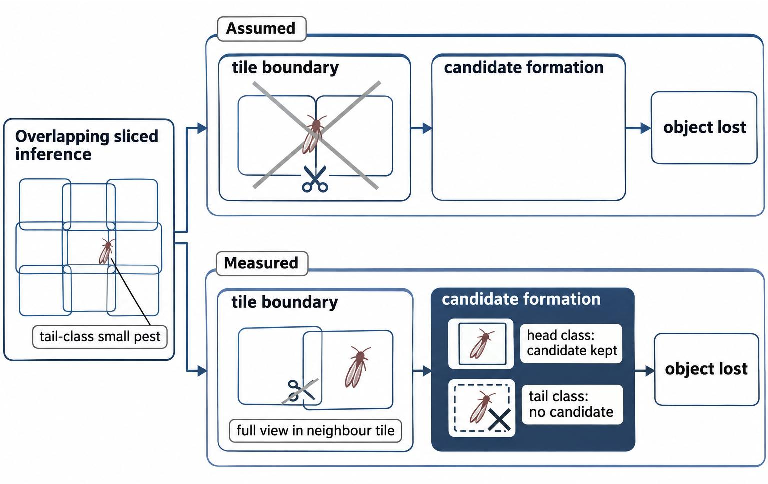
\includegraphics[width=0.98\textwidth,height=0.8\textheight,keepaspectratio]{figures/fig_roadmap.pdf}
  \caption{Assumed slice-boundary loss versus measured loss at candidate formation for tail-class small pests.}
  \label{fig:roadmap}
\end{figure}

% ---- appendix FCOS supplements (data figures, FCOS analogs of Figs partition / stage-survival;
%      PDFs produced by the experiment-bridge step, include block added by paper-figure-html to keep latex_includes complete) ----
\begin{figure}[!htbp]
    \centering
    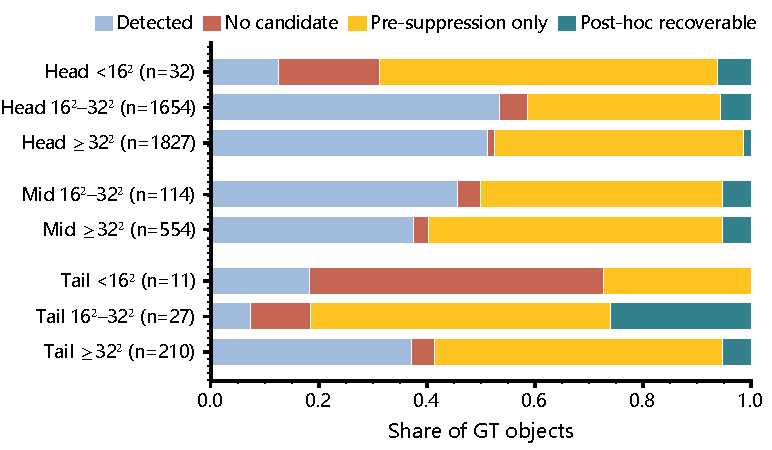
\includegraphics[width=0.98\textwidth,height=0.8\textheight,keepaspectratio]{figures/fig_partition_fcos.pdf}
    \caption{Recovery-ceiling partition of every audit object under the second detector (FCOS-ResNet50-FPN, SAHI $T$=320, overlap 0.25, frozen GREEDYNMM-IOS merge). Categories and layout match Fig.~\ref{fig:partition}; the cross-detector contrast shows the dominant loss stage is detector-dependent (K4).}
    \label{fig:partition-fcos}
\end{figure}

\begin{figure}[!htbp]
    \centering
    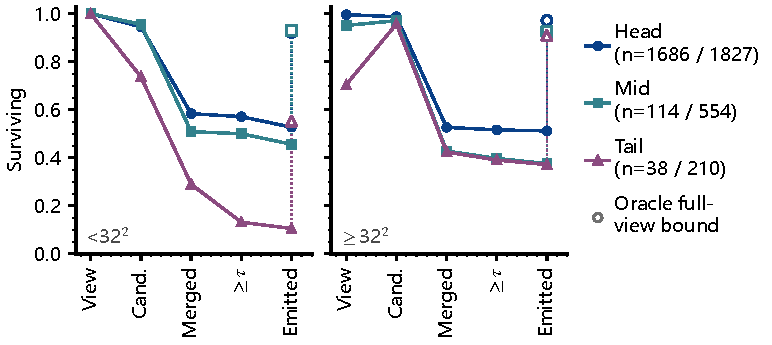
\includegraphics[width=0.98\textwidth,height=0.8\textheight,keepaspectratio]{figures/fig_stage_survival_fcos.pdf}
    \caption{Stage-survival profile of the per-object ledger on the audit set under FCOS-ResNet50-FPN (SAHI $T$=320, overlap 0.25). Axes match Fig.~\ref{fig:stage-survival}: left, objects smaller than $32^2$; right, larger objects; hollow markers are the oracle full-view read-out.}
    \label{fig:stage-survival-fcos}
\end{figure}
